\section{Theoretical Analysis}
\label{sec:analysis}

In this section, the circuit shown in \textbf{Figure~\ref{fig:diagram_t4}} is analysed
theoretically.
\begin{figure}[h] \centering
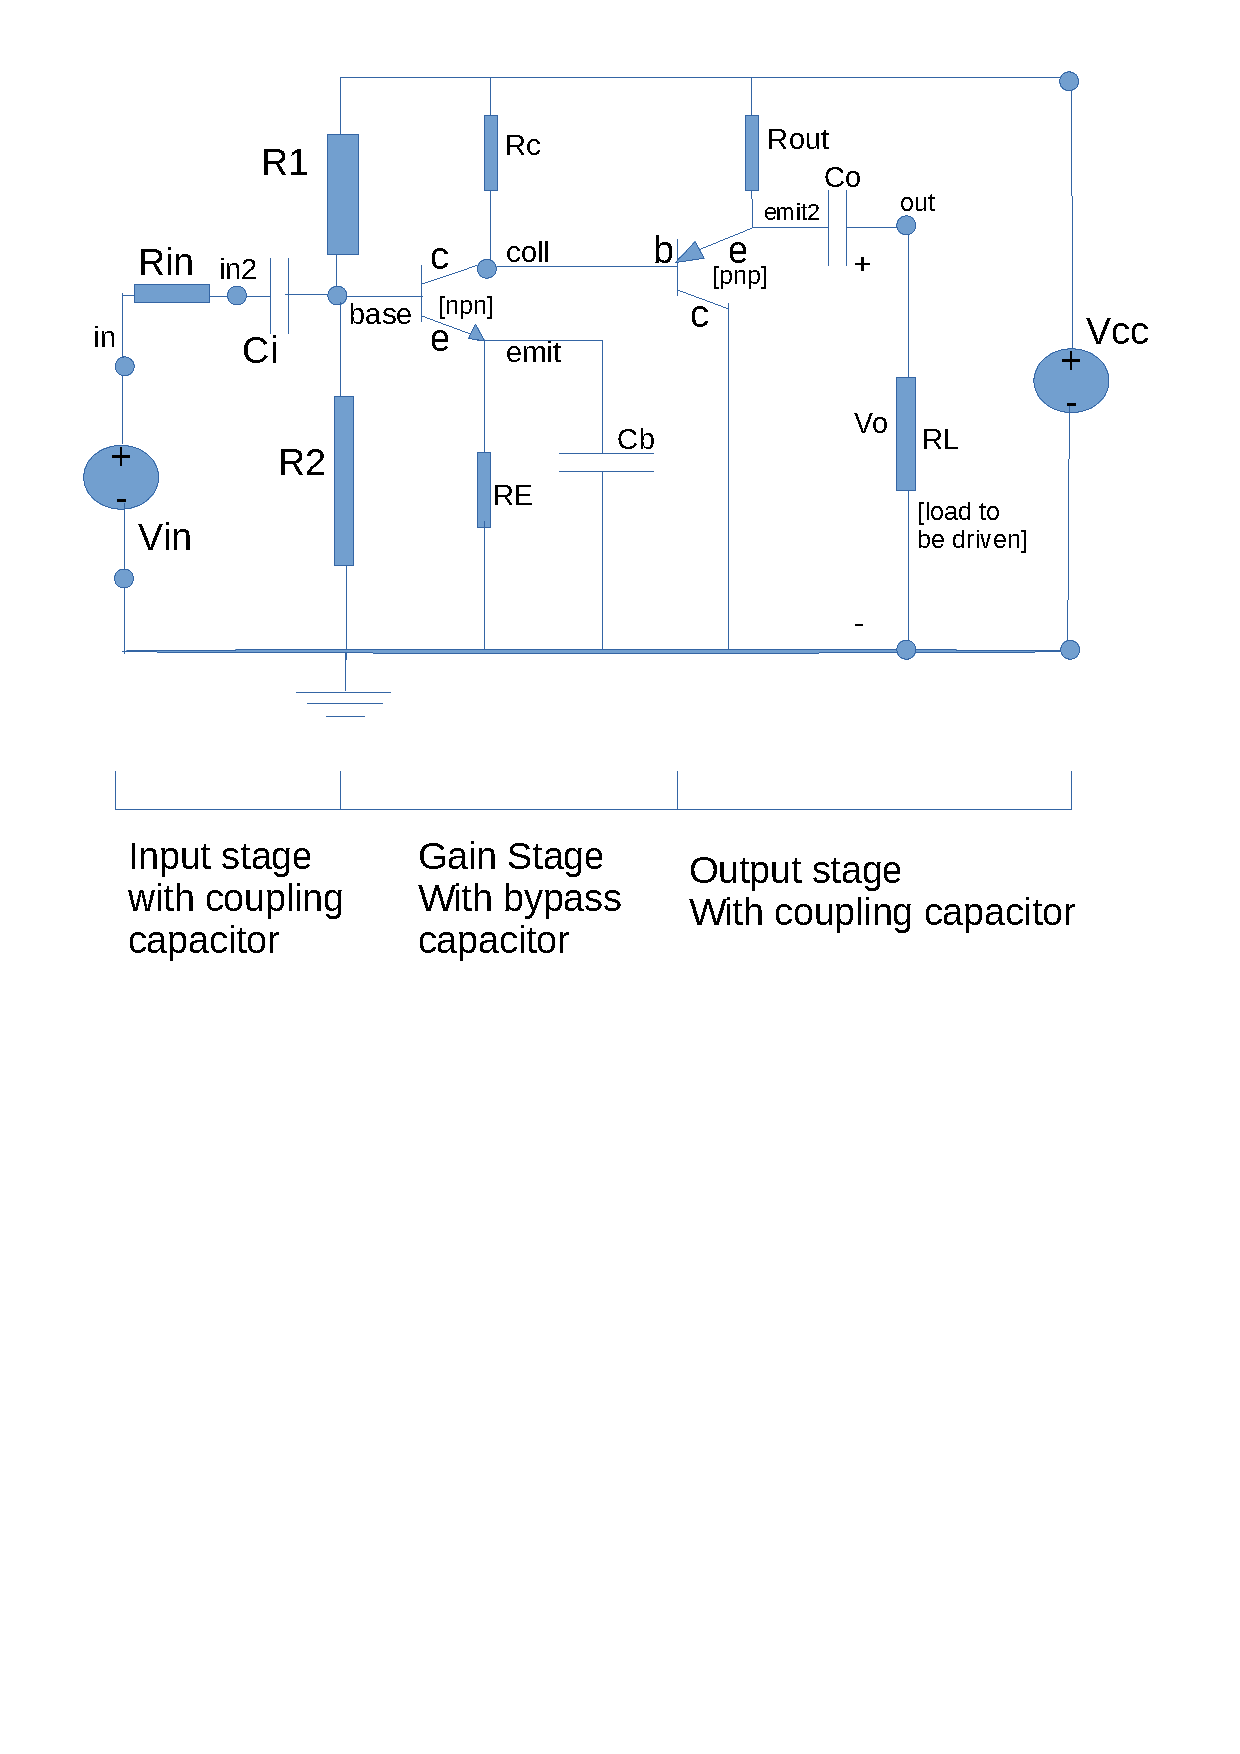
\includegraphics[width=0.95\linewidth]{diagram_t4.pdf}
\vspace{-7cm}
\caption{Diagram of the circuit considered for the computations and simulations.}
\label{fig:diagram_t4}
\end{figure}


As explained before, in the previous section, the audio amplifier is composed of two stages. In the first stage (the gain stage) the primary objective is to amplify the voltage input signal. To do so this section will have a high gain. This stage also has a high input impedance which avoids the degradation of the input signal. The  downside of this stage is its high output impedance that makes it difficult to connect to a speaker without having the signal degrade in the exit. That is why there is an output stage. This stage will have a low output impedance which is very good because it allows us to connect to the speaker while minimizing signal degradation. When we connect the two stages the signal does not degrade very much beacause the output stage input impedance is higher than the output impedance of the gain stage, meaning little or no signal degradation in the transition between stages. This can be seen in one of the following tables. In the output stage the gain is very close to one, meaning than there will be no amplification nor attenuation of the signal.\par  

The main purpose of the bypass capacitor $C_{E}$ in the gain stage is to avoid a gain loss through resistor ${R_E}$ and the main purpose of resistor ${R_E}$ is to stabilize the temperature effect. In  DC the temperature effect is most important while in AC the gain is most important . Therefore there needs to be an equilibrium. This components were placed in parallel in order to achive this equilibrium. For lower frequencies (DC) capacitor $C_{E}$ behaves like an open circuit and the current goes through resistor ${R_E}$, stabilizing the temperature effect. For higher frequencies (AC) the capacitor is a short circuit and therefore it is used to bypass the resistor $R_{E}$, avoiding lowering the gain (gain is stable in the desired passband).\par


The human ear perceives frequencies between 20 Hz to 20 kHz and therefore we should chose coupling capacitors that behave like short-circuits for these frequencies, as the coupling capacitors affect the lower cutoff frequency and consequently the bandwidth. The final values considered for the circuit parameters (as named in the above figure) were the following:

\hfill
 \parbox{1\linewidth}{
  \centering
  \begin{tabular}{|l|l|l|r|}
    \hline    
    {\bf Parameter} & {\bf Value} & {\bf Units }\\ \hline
    \input{valores.tex}
  \label{tab:params}
  \end{tabular}
  }
\par

In the following table is the operating point analysis, both for the theoretical analysis (right) and the Ngspice simulation (left), in order to make a side-by-side comparison. This also includes a flag (last row) that ensures that both BJTs are in the Forward Active Region - if everything is ok, the flag should read "ok". If any (or both) of the transistor are not in this region, the flag should read "bad". The condition considered was, for the NPN transistor: $V_{CE} > V_{BE} <=> V_{C} > V_{B}$ and for the PNP transistor: $V_{EC} > V_{EB} <=> V_{C} < V_{B}$.\par

\hfill
 \parbox{1\linewidth}{
  \centering
  \begin{tabular}{|l|l|l|r|}
    \hline    
    {\bf Node Voltage} & {\bf Simulation} & {\bf Theoretical } & {\bf Units }\\ \hline
    Vbase & 1.3841 & 1.3841 & V\\ \hline
Vcoll & 8.6547 & 8.6547 & V\\ \hline
Vemit & 0.6855 & 0.6855 & V\\ \hline
Vemit2 & 9.3974 & 9.3974 & V\\ \hline
Vin & 0.0000 & 0.0000 & V\\ \hline
Vin2 & 0.0000 & 0.0000 & V\\ \hline
Vout & 0.0000 & 0.0000 & V\\ \hline
Vvcc & 12.0000 & 12.0000 & V\\ \hline

  \label{tab:op_FAR}
  \end{tabular}
  }
\par
The circuit used to compute the lower cutoff frequency and the gain, theoretically, was the following incremental model (which includes the coupling capacitors given that these are the limiting factors in terms of the lower cutoff frequency). For the upper cutoff frequency it is a little bit more complex given that this is due to the parasitic capacitances of the transistor, which are part of the Ngspice model, but were not considered in the theory.\par 

\begin{figure}[h] \centering
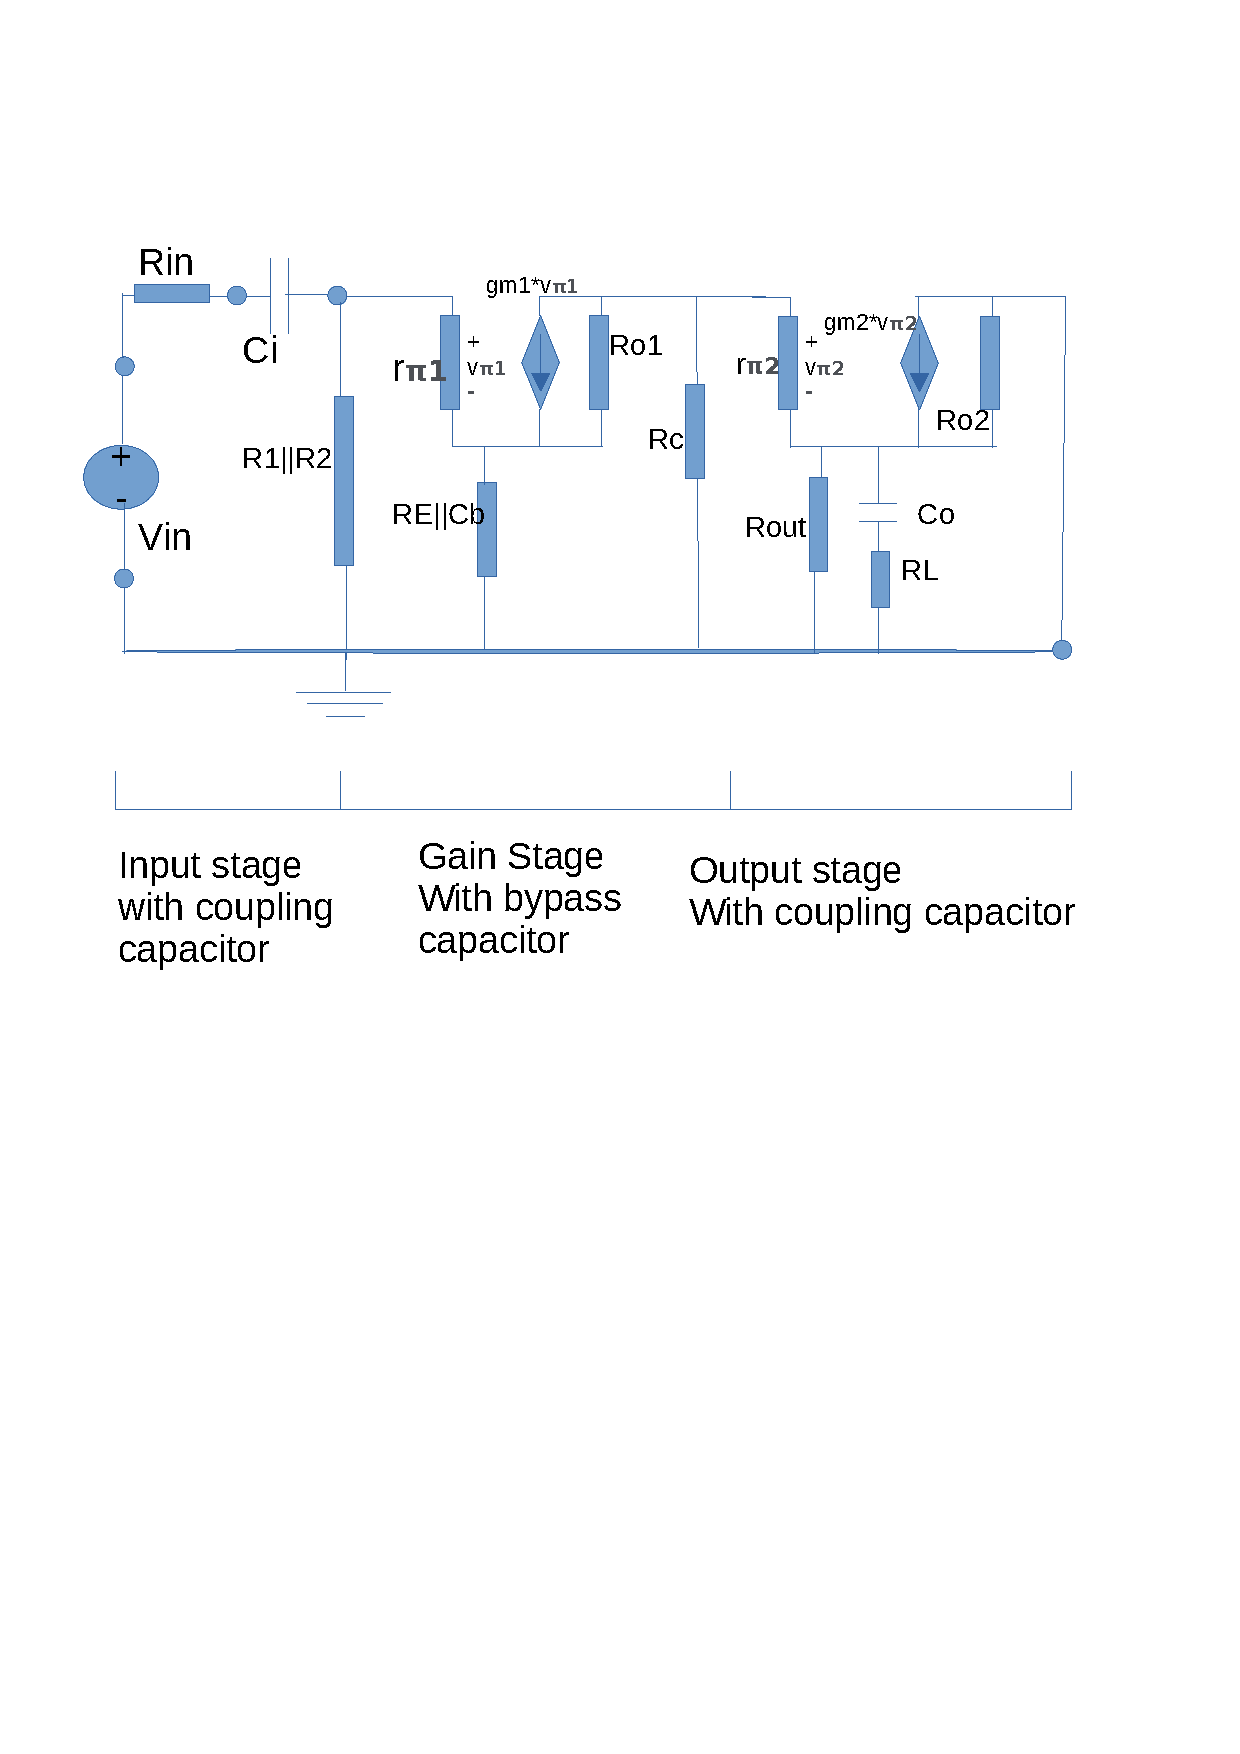
\includegraphics[width=0.95\linewidth]{incremental_t4.pdf}
\vspace{-7cm}
\caption{Diagram of the incremental model considered for the gain and frequency response computations.}
\label{fig:diagram_t4}
\end{figure}
\par
\vspace{1cm}


The gain of the audio amplifier, the upper and lower cut off frequency, the bandwidth and the input and output impedances as well as the merit are presented in the following table, both for the theoretical analysis (right) and the Ngspice simulation (left), in order to make a side-by-side comparison.\par


\hfill
 \parbox{1\linewidth}{
  \centering
  \begin{tabular}{|l|l|l|r|}
    \hline    
    {\bf Parameter} & {\bf Simulation} & {\bf Theoretical } & {\bf Units }\\ \hline
    Zi & 766.402 & 640.49 & Ohm\\ \hline
Zo & 4.49605 & 2.9364 & Ohm\\ \hline
Cost & 8116 & Cost & MU\\ \hline
uco & 3106933.000 & 2123123123123.000 & Hz\\ \hline
lco & 7.924 & 2123123123123.000 & Hz\\ \hline
Bandwidth & 3106925.076 & 2123123123123.000 & Hz\\ \hline
Gainv(out) & 56.041 & -107.220 & [adimensional]\\ \hline
MERIT & 2707.5316 & -104.2260 & gold medals\\ \hline

  \label{tab:results}
  \end{tabular}
  }
  
  
There was some discrepancy here; for starters note that the input and output impedances for the intermediate stages were not simulated, they were only calculated in theory. The same goes for the gain of the intermediate stages. On a final note, the total input and output impedances of the amplifier were quite different in the two scenarios (theory vs simulation), but of the same order of magnitude; the only other significant difference was the lower cut off frequency.\par

Do note that the upper cutoff frequency here used in the theoretical column was actually obtained from Ngspice: to calculate this frequency in theory, we would need to take into account the parasitic capacitances in the transistor, which proved to be quite more complex and therefore was not used.


  The next figures present the plot of gain obtained in the theoretical analysis.

%In \textbf{Table~\ref{tab:theoretical}} the values for the branch currents and the node voltages obtained from the Octave script for both methods are presented. Here, the node voltages in the mesh method were computed from the respective currents, which were determined as described in the previous subsectio

\begin{figure}[H] \centering
\includegraphics[width=0.6\linewidth]{gain_octave.pdf}
\caption{Output voltage gain of the audio amplifier as a function of frequency}
\label{fig:gain_octa}
\end{figure}




\pagebreak


